\chapter{Fizibilite}

Bu bölümde projenin olabilirlik etüdü yapılmaktadır. Projenin teknik, zaman, yasal ve ekonomik fizibilitesi incelenmektedir.

\section{Teknik Fizibilite}
Projenin teknik fizibilitesi, yazılım fizibilitesi ve donanım fizibilitesi olmak üzere iki ayrı başlık altında işlenmiştir.

\subsection{Yazılım Fizibilitesi}
Geliştirilen uygulamanın iPhone cihazlarda çalışacak olması sebebiyle iOS işletim sistemi tercih edilmiştir. Projenin geliştirilmesi için XCode geliştirici ortamı kullanılmıştır. iOS işletim sistemi için geliştirilen uygulamalar sadece XCode geliştirici ortamında gerçekleştirilebilmektedir. Apple tarafından yapılan bu kısıtlama sebebiyle XCode kullanılmıştır. 
Projeyi geliştirirken kullanılacak programlama dili ise iOS işletim sistemi tarafından desteklenen, yeni, esnek ve anlaşılabilir bir programlama dili olan Swift dilidir. Objective - C karmaşık ve eski bir programlama dili olması sebebiyle projenin geliştirilme aşamasında kullanılmamıştır.
Veritabanı aracı olarak ise XCode ortamı ile beraber gelen CoreData sistemi kullanılmıştır. iOS işletim sistemleri üzerinde Swift programlama dili ile beraber oldukça verimli çalışan bir veritabanı sistemidir. Projenin makine öğrenmesi kısmında ise açık kaynak kodlu bir araç olan Weka  kullanılmıştır. Açık kaynak kodlu ve basit ara yüzü sebebiyle tercih edilmiştir.

\subsection{Donanım Fizibilitesi}
Proje, iPhone cihazlar üzerinde çalışmak üzere tasarlanmıştır. Verilerin elde edildiği iki tür sensör bulunmaktadır. İvmeölçer (Accelerometer) ve jiroskop (Gyroscope). Projede verileri elde etmek için kullanılan cihazın teknik özellikleri
\begin{itemize}
  \item 64 bit A8 Mikroişlemci
  \item M8 Hareket İşlemcisi
  \item 1GB RAM
  \item 16GB Disk Kapasitesi
\end{itemize}

Projenin gerçekleştirildiği bilgisayara ait teknik özellikler
\begin{itemize}
  \item 2.4 GHz Intel Core i5 İşlemci
  \item 8GB RAM
  \item Intel Iris 1536 HD Grafik Kartı
  \item 256GB SSD Disk Kapasitesi
\end{itemize}

Proje iOS 10 yüklü , ivmeölçer ve jiroskop bulunan tüm iPhone cihazlarda çalışabilecek şekilde tasarlandı.

\section{Zaman Fizibilitesi}
\begin{figure}[!htbp]
\centering
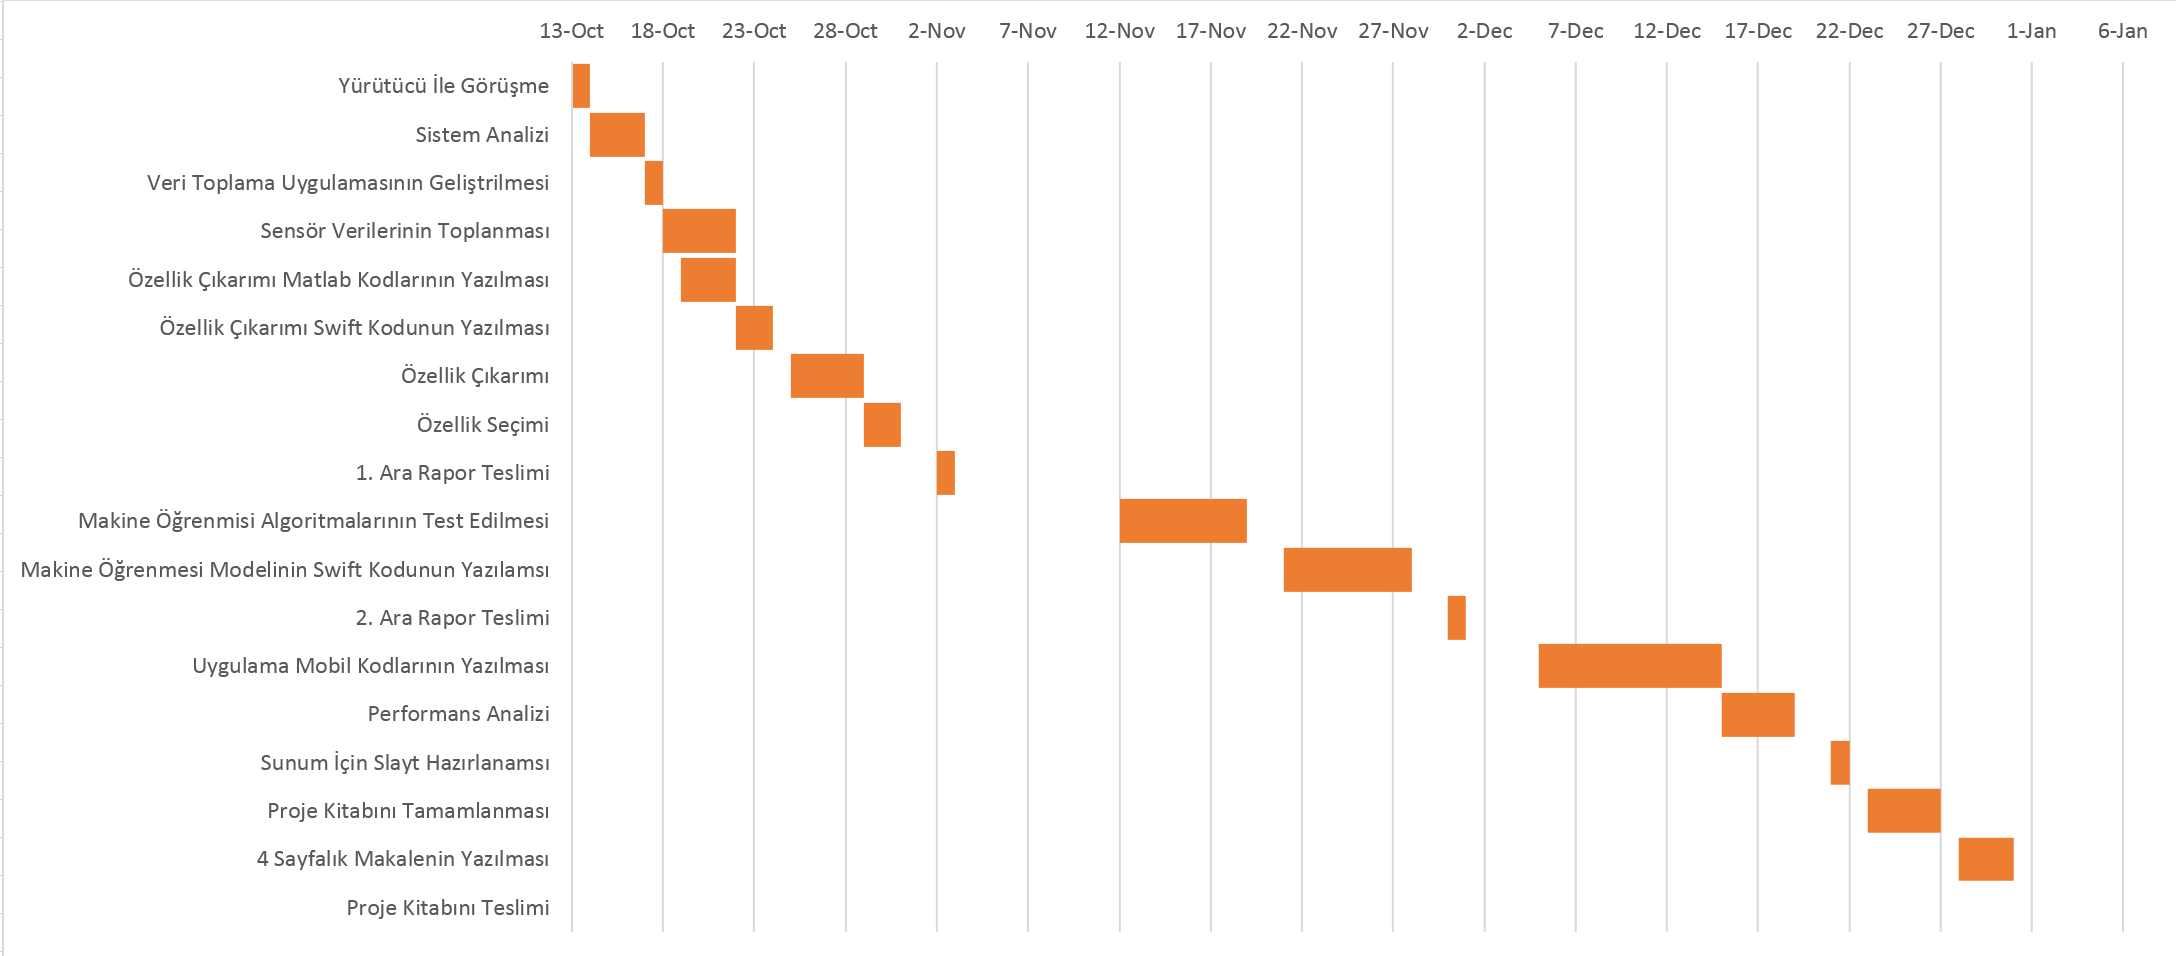
\includegraphics[width=\textwidth]{projectChapters/images/gantt.png}
\caption{Zaman fizibilitesine ait Gantt diyagramı}
\end{figure}

\section{Yasal Fizibilite}
Geliştirilmekte olunan proje mevcut kanun ve yükümlülüklere uygun olup, herhangi bir patent vb. korunmuş hakkı 
ihlal etmemektedir
\newpage
\section{Ekonomik Fizibilite}
Proje kapsamında kullanılan yazılım teknolojileri ücretsiz olup sisteme ek bir maliyet getirmemektedir. Bu sistemi geliştirmek için gerekli olan donanım maliyeti Tablo 3.1 ‘deki gibidir. Çalışan maliyeti Tablo 3.2 ‘deki gibidir. Sensör verilerinin toplanması için gerekli olan Ulaşım Giderleri Tablo 3.3 ' deki gibidir.
\begin{table}[!h]
\centering
\caption{Donanım Giderleri}
\begin{tabular}{|l|r|}
\hline
\textbf{Cihaz}           & \textbf{Fiyat (TL)}     \\ \hline
Kişisel Bilgisayar       & 3.500                   \\ \hline
Test Telefonu            & 2.000                   \\ \hline
\textit{\textbf{Toplam}} & \textit{\textbf{5.500}} \\ \hline
\end{tabular}
\end{table}

\begin{table}[!h]
\centering
\caption{Çalışan Giderleri}
\begin{tabular}{|l|r|r|r|}
\hline
\textbf{Görev}  & \textbf{Süre (Ay)} & \textbf{Aylık Ücret} & \textbf{Toplam Gider (TL)} \\ \hline
Makine Öğrenmesi Modeli Oluşturma & 3                  & 1.500                 & 4.500                       \\ \hline
iOS Mobil Uygulama Geliştirme & 1                  & 2.500                 & 2.500                       \\ \hline
\end{tabular}
\end{table}

\begin{table}[!h]
\centering
\caption{Ulaşım Giderleri}
\begin{tabular}{|l|r|r|}
\hline
\textbf{Ulaşım Türü}     & \textbf{Fiyat (TL)}   & \textbf{Süre (Dk)}    \\ \hline
Metro                    & 10                    & 40                    \\ \hline
Hafif Raylı              & 10                    & 40                    \\ \hline
Metrobüs                 & 12                    & 40                    \\ \hline
Marmaray                 & 10                    & 40                    \\ \hline
Otobüs                   & 5                     & 45                    \\ \hline
Tramvay                  & 10                    & 40                    \\ \hline
Araba                    & 60                    & 45                    \\ \hline
\textit{\textbf{Toplam}} & \textit{\textbf{117}} & \textit{\textbf{290}} \\ \hline
\end{tabular}
\end{table}

\begin{table}[!h]
\centering
\caption{Toplam Gider}
\begin{tabular}{|l|r|}
\hline
\textbf{Gider}           & \textbf{Fiyat (TL)}     \\ \hline
Donanım Giderleri        & 5.500                    \\ \hline
Yazılım Giderleri        & 0                       \\ \hline
Çalışan Giderleri        & 7.000                    \\ \hline
Ulaşım Giderleri         & 112                     \\ \hline
\textit{\textbf{Toplam}} & \textit{\textbf{12.612}} \\ \hline
\end{tabular}
\end{table}